% 
% Permission is granted to copy, distribute and/or modify this document
% under the terms of the GNU Free Documentation License, Version 1.2
% or any later version published by the Free Software Foundation;
% with no Invariant Sections, no Front-Cover Texts, and no Back-Cover
% Texts.  A copy of the license is included in the section entitled "GNU
% Free Documentation License".

\documentclass[11pt]{article}

\usepackage{OTSubset_Documentation}
\usepackage{Math_Notations}

\makeindex

\begin{document}

\thispagestyle{empty}

% 
% Permission is granted to copy, distribute and/or modify this document
% under the terms of the GNU Free Documentation License, Version 1.2
% or any later version published by the Free Software Foundation;
% with no Invariant Sections, no Front-Cover Texts, and no Back-Cover
% Texts.  A copy of the license is included in the section entitled "GNU
% Free Documentation License".
\vspace*{2cm}

\begin{center}
  {\huge \bf Documentation of the OpenTURNS-Subset module}
  \input{GenericInformation.tex}
\end{center}



\newpage
%  
%  Permission is granted to copy, distribute and/or modify this document
%  under the terms of the GNU Free Documentation License, Version 1.2
%  or any later version published by the Free Software Foundation;
%  with no Invariant Sections, no Front-Cover Texts, and no Back-Cover
%  Texts.  A copy of the license is included in the section entitled "GNU
%  Free Documentation License".
\vspace{0.5in}
\begin{center}
\vspace{0.3in}
\emph{\fontshape{sc} Abstract}
\vspace{0.5in}
\end{center}

The purpose of this document is to present the OpenTURNS-Subset module.

This document is organized according to the OpenTURNS documentation:
\begin{itemize}
\item a \itshape{Reference Guide} which gives some theoretical basis,
\item the \itshape{Use Cases Guide} which details scripts in python and helps the User to learn as quickly as possible the manipulation of the $subset$ module,
\item the \itshape{User Manual} which details the $subset$ objects and give the list of their methods,
\item a \itshape{Validation Note} which benchmarks the numerical methods available in the module,
\item the \itshape{Architecture Guide} which describes the design of the classes and their role.
\end{itemize}


\tableofcontents
\newpage
% 
% Copyright 2009-2012 Phimeca

%%%%%%%%%%%%%%%%%%%%%%%%%%%%%%%%%%%%%%%%%%%%%%%%%%%%%%%%%%%%%%%%%%%%%%%%%%%%%%%%%%%%%%%%%% 



\section{Reference Guide}

\subsection{Subset Simulation}

\MathematicalDescription{
\underline{\textbf{Goal}}\\
Let us note $\mathcal D_f = \{\ux \in \mathbb R^{n_X} | g(\ux,\underline{d}) \leq 0\}$.
The goal is to estimate the following probability:
\begin{eqnarray*}
        P_f &=& \int_{\mathcal D_f} f_{\uX}(\ux)d\ux\\
            &=& \int_{\mathbb R^{n_X}} \mathbf{1}_{\{g(\ux,\underline{d}) \:\leq 0\: \}}f_{\uX}(\ux)d\ux\\
            &=& \Prob {\{g(\uX,\underline{d}) \leq 0\}}
\end{eqnarray*}

\underline{\textbf{Principles}}\\
 The idea of the Subset Sampling method is to replace simulating a rare failure event in the original probability space by a sequence of simulations of more frequent conditional events $F_i$ 
\begin{eqnarray*}
  F_1 \supset F_2 \supset \dots \supset F_m = F
\end{eqnarray*}
The original probability estimate rewrites
\begin{eqnarray*}
  P_f = P(F_m) = P(\bigcap \limits_{i=1}^m F_i) = P(F_1) \prod_{i=2}^m P(F_i|F_{i-1})
\end{eqnarray*}
And each conditional subset failure region is chosen by setting the threshold $g_i$ so that $P(F_i|F_{i-1})$ leads to a conditional failure probability of order $0.1$\\
\begin{eqnarray*}
  F_i =\Prob {\{g(\uX,\underline{d}) \leq g_i\}}
\end{eqnarray*}
The conditional samples are generated by the means of Markov Chains, using the Metropolis Hastings algorithm. 

\underline{\textbf{Coefficient of variation}}\\
$N$ being the number of simulations per subset, and $p_{0i}$ the conditional probability of each subset event, and $\gamma_i$ the autocorrelation between Markov chain samples.
\begin{eqnarray*}
  \delta^2 = \sum_{i=1}^m \delta^2_i = \sum_{i=1}^m (1+\gamma_i) \frac{1-p_{0i}}{p_{0i}N}
\end{eqnarray*}
The first event $F_1$ not being conditional, $\delta^2_1$ expresses as the classic Monte Carlo c.o.v.
}
{
% Autres notations et appellations
}

\Methodology{
This method is part of the step C of the global methodology. It requires the specification of the joined probability density function of the input variables and the value of the threshold and the comparison operator.\\
}
{
$p0$ being the same conditional probability for each level, the number of steps is given by 
\begin{eqnarray*}
   m = \frac{\log P_f}{\log p0}
\end{eqnarray*}
The total number of samples required to reach a c.o.v. of $\delta$ in the global probability estimate can be approximated by
\begin{eqnarray*}
  N_T \approx m N = |\log P_f|^r \frac{(1+\gamma)(1-p_0)}{p_0|\log p_0|^r \delta^2}
\end{eqnarray*}

So the subset simulation shows a substantial improvement ($N_T \sim \log P_f$) compared to crude Monte Carlo ($N_T \sim \frac{1}{P_f}$) sampling when estimating rare events.

\vspace{10mm}
The following references are a first introduction to the subset simulation method:\\

\label{ab01} S.K. Au and J. L. Beck \textit{Estimation of small failure probabilities in high dimensions by subset simulation}. In Probabilistic Engineering Mechanics 16, 2001

}

\newpage
% 
% Permission is granted to copy, distribute and/or modify this document
% under the terms of the GNU Free Documentation License, Version 1.2
% or any later version published by the Free Software Foundation;
% with no Invariant Sections, no Front-Cover Texts, and no Back-Cover
% Texts.  A copy of the license is included in the section entitled "GNU
% Free Documentation License".




%%%%%%%%%%%%%%%%%%%%%%%%%%%%%%%%%%%%%%%%%%%%%%%%%%%%%%%%%%%%%%%%%%%%%%%%%%%%%%%%%%%%%%%%%% 
\section{Use Cases Guide}

This section presents the main functionalities of the module $subset$ in their context.



%%%%%%%%%%%%%%%%%%%%%%%%%%%%%%%%%%%%%%%%%%%%%%%%%%%%%%%%%%%%%%
\subsection{Which python modules to import ?}

In order to use the functionalities described in this documentation, it is necessary to import  : 
\begin{itemize}
   \item the $otsubset$ module.
\end{itemize}

Python  script for this use case :
\begin{lstlisting}
from otsubset import *
\end{lstlisting}



\subsection{Create a subset simulation algorithm}

Details on the SubsetSampling object can be found in the UserManual at the next chapter.\\

Details on simulation algorithms can be found in the Reference Guide (\href{OpenTURNS_ReferenceGuide.pdf}{see files Reference Guide - Step C -- Estimating the probability of an event using Sampling} and files around).\\


\requirements{
  \begin{description}
  \item[$\bullet$] the event we want to evaluate the probability : {\itshape myEvent}
  \item[type:] Event
  \item[$\bullet$] the target conditional probability of each subset domain
  \item[type:] NumericalScalar
  \item[$\bullet$] the width of the MCMC random walk uniform distribution
  \item[type:] NumericalScalar
  \item[$\bullet$] the number of samples per step
  \item[type:] UnsignedLong
  \end{description}
}
{
  \begin{description}
  \item[$\bullet$] the SubsetSampling simulation algorithm : {\itshape mySSAlgo}
  \item[type:] Simulation
  \item[$\bullet$] the SubsetSampling simulation result : {\itshape myResult}
  \item[type:] SimulationResult
  \end{description}
}

\newpage
Python  script for this UseCase :

\begin{lstlisting}
  # Create a Subset Sampling algorithm
  mySSAlgo = SubsetSampling(myEvent)

  # Change the target conditional probability of each subset domain
  # mySSAlgo.setTargetProbability(0.9)

  # Set the width of the MCMC random walk uniform distribution
  mySSAlgo.setProposalRange(1.8)

  # This allows to control the number of samples per step
  mySSAlgo.setMaximumOuterSampling(10000)

  # Run the algorithm
  mySSAlgo.run()

  # Retrieve the result
  myResult = mySSAlgo.getResult()
  
  # Extract some results
  print 'Pf:', myResult.getEventProbability()
  print 'Cov:', myResult.getCoefficientOfVariation()
  print 'Number of steps:', myResult.getNumberOfSteps()
\end{lstlisting}


\newpage
% 
% Permission is granted to copy, distribute and/or modify this document
% under the terms of the GNU Free Documentation License, Version 1.2
% or any later version published by the Free Software Foundation;
% with no Invariant Sections, no Front-Cover Texts, and no Back-Cover
% Texts.  A copy of the license is included in the section entitled "GNU
% Free Documentation License".

%%%%%%%%%%%%%%%%%%%%%%%%%%%%%%%%%%%%%%%%%%%%%%%%%%%%%%%%%%%%%%%%%%%%%%%%%%%%%%%%%%%%%%%%%% 
\section{User Manual}

This section gives an exhaustive presentation of the objects and functions provided by the $subset$ module, in the alphabetic order.

\subsection{SubsetSampling}

This class inherits from the Simulation class, please refer to the Simulation class documentation for common methods.\\
Note that this algorithm cannot be controlled by means of a maximum coefficient of variation.\\

\begin{description}

  \item[Usage :] \rule{0pt}{1em}
    \begin{description}
    \item $SubsetSampling(event)$
    \item $SubsetSampling(event, proposalRange)$
    \item $SubsetSampling(event, proposalRange, targetProbability)$
    \end{description}

  \item[Arguments :]  \rule{0pt}{1em}
    \begin{description}
    \item $event$ : an Event, the event we want to compute the probability of
    \item $proposalRange$ : a NumericalScalar, the range of the uniform proposal as distribution of the random walk (default$=2.0$)
    \item $targetProbability$ : a NumericalScalar, the probability estimate of each conditional domain $P(F_i|F_{i-1})$ (default$=0.1$)
    \end{description}

  \item[Value :] a SubsetSampling

  \item[Details :]  \rule{0pt}{1em}
    \begin{description}
    \item Like all the simulation algorithms, the number of samples per step is determined by $maximumOuterSampling*blockSize$ (default $1000 \times 1$)
    \item Like usual, use the $getResult$ method to access the computed results.
    \end{description}

  \item $getProposalRange$
    \begin{description}
    \item[Usage :] $getProposalRange()$
    \item[Arguments :] no argument
    \item[Value :] a NumericalScalar, the range of the uniform proposal as distribution of the random walk
    \end{description}
    \bigskip

  \item $getTargetProbability$
    \begin{description}
    \item[Usage :] $getTargetProbability()$
    \item[Arguments :] no argument
    \item[Value :] a NumericalScalar, the probability estimate of each conditional domain $P(F_i|F_{i-1})$
    \end{description}
    \bigskip

  \item $getNumberOfSteps$
    \begin{description}
    \item[Usage :] $getNumberOfSteps()$
    \item[Arguments :] no argument
    \item[Value :] an UnsignedLong, the number of subset steps
    \end{description}
    \bigskip

  \item $getThresholdPerStep$
    \begin{description}
    \item[Usage :] $getThresholdPerStep()$
    \item[Arguments :] no argument
    \item[Value :] a NumericalPoint, the intermediate threshold values
    \end{description}
    \bigskip

  \item $getGammaPerStep$
    \begin{description}
    \item[Usage :] $getGammaPerStep()$
    \item[Arguments :] no argument
    \item[Value :] a NumericalPoint, the intermediate autocorrelation values
    \end{description}
    \bigskip  
    
   \item $getCoefficientOfVariationPerStep$
    \begin{description}
    \item[Usage :] $getCoefficientOfVariationPerStep()$
    \item[Arguments :] no argument
    \item[Value :] a NumericalPoint, the intermediate c.o.v. values
    \end{description}
    \bigskip  
      
  \item $getProbabilityEstimatePerStep$
    \begin{description}
    \item[Usage :] $getProbabilityEstimatePerStep()$
    \item[Arguments :] no argument
    \item[Value :] a NumericalPoint, the intermediate pf values
    \end{description}
    \bigskip 
    
  \item $setKeepEventSample$
    \begin{description}
    \item[Usage :] $setKeepEventSample(keepEventSample)$
    \item[Arguments :] a boolean keepEventSample, deciding whether we keep the event samples
    \item[Value :] none
    \end{description}
    \bigskip   
    
  \item $getEventInputSample$
    \begin{description}
    \item[Usage :] $getEventInputSample()$
    \item[Arguments :] no argument
    \item[Value :] a NumericalSample, the input sample values. See $setKeepEventSample$.
    \end{description}
    \bigskip 
    
  \item $getEventOutputSample$
    \begin{description}
    \item[Usage :] $getEventOutputSample()$
    \item[Arguments :] no argument
    \item[Value :] a NumericalSample, the output sample values. See $setKeepEventSample$.
    \end{description}
    \bigskip 
    
The methods $getProposalRange$, $getTargetProbability$ have their corresponding $setMethod$.

\item[Links] \rule{0pt}{1em}
\end{description}


\newpage \subsection{SubsetSamplingResult}

This class inherits from the SimulationResultImplementation class, please refer to the SimulationResult class documentation for common methods, \dots \\
Note that the $outersampling$ result can exceed the algorithms $maximumOuterSampling$, as the total number of samples is determined by the number of steps, so that 
$outersampling = maximumOuterSampling \times numberOfSteps$.\\


\newpage
% 
% Copyright 2009-2012 Phimeca


%%%%%%%%%%%%%%%%%%%%%%%%%%%%%%%%%%%%%%%%%%%%%%%%%%%%%%%%%%%%%%%%%%%%%%%%%%%%%%%%%%%%%%%%%% 
\section{Validation}

This section aims at exposing academical benchmarks from which the numerical methods can be guaranteed as robust.\\
We will focus on showing the accuracy int the case of low probabilities, and also exposing that the result is reached for the same cov at a lower limit-state evaluation cost.\\
The method will be compared to crude MC on various benchmarks for which we will expose the number of samples $N$, the failure probability $P_F$, the associated reliability inde $\beta$ and the coefficient of variation $Cov$.\\

\subsection{R-S}

The classical constraint-resistance example and the associated results are gathered from F. Deheeger \textit{Couplage mecano-fiabiliste : $^2$SMART - methodologie d'apprentissage en fiabilite}.

\subsubsection{Problem statement}

$
\begin{array}{lrrr}
Variable & Distribution & Mean & \text{Standard deviation} \\
\hline
R & Normal   & 7. & 1.0 \\
S & Normal   & 2. & 1.0 \\
\end{array}
$
\vspace{10mm}


Limit-state:\\
\begin{eqnarray*}
  g = R - S\\
  g < 0
\end{eqnarray*}

\subsubsection{Results}

$
\begin{array}{cccc}
            & Exact & MC & Subset \\
\hline
N & - & 10^6   & 4 \times 10^4 \\
P_F & 2.0\times10^{-4} & 2.2 \times10^{-4}  & 2.03 \times10^{-4}\\
\beta & 3.54 & 2.86  & 3.537 \\
Cov & - & 0.08  & 0.086 \\
\end{array}
$



\newpage
\subsection{Waarts system series}

The waarts test is taken from P. H. Waarts \textit{Structural reliability using finite element analysis}, 2000.

\subsubsection{Problem statement}

$
\begin{array}{lrrr}
Variable & Distribution & Mean & \text{Standard deviation} \\
\hline
u1 & Normal   & 0. & 1.0 \\
u2 & Normal   & 0. & 1.0 \\
\end{array}
$
\vspace{10mm}

Limit-state:\\
\begin{eqnarray*}
  g1 = 0.1 * (u1 - u2)^2 - \frac{u1 + u2}{\sqrt{2}} + 3\\
  g2 = 0.1 * (u1 - u2)^2 + \frac{u1 + u2}{\sqrt{2}} + 3\\
  g3 = 3.0, u1 - u2 + 3.5 \sqrt{2}\\
  g4 = -u1 + u2 + 3.5 \sqrt{2}\\
  g = min(g1, g2, g3, g4)\\
  g < 0
\end{eqnarray*}


\subsubsection{Results}

$
\begin{array}{ccc}
            & MC & Subset \\
\hline
N & 10^6   & 4\times 10^4 \\
P_F & 2.216 \times10^{-3}  & 2.106 \times10^{-3} \\
\beta & 2.86 & 2.862 \\
Cov & 0.021  & 0.06348 \\
\end{array}
$


\newpage
% 
% Copyright 2009-2012 Phimeca

%%%%%%%%%%%%%%%%%%%%%%%%%%%%%%%%%%%%%%%%%%%%%%%%%%%%%%%%%%%%%%%%%%%%%%%%%%%%%%%%%%%%%%%%%% 
\section{Architecture guide}

This document makes up the general specification design for the architecture of the Subset module.

\begin{figure}[htb]
  \begin{center}
    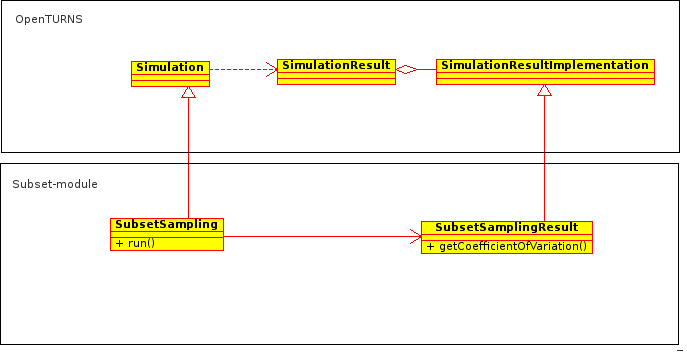
\includegraphics[scale=0.8]{architecture.png}
    \caption{Subset module classes.}\label{fig:architecture}
  \end{center}
\end{figure}


\paragraph{SubsetSampling}

The class SubsetSampling derives from the Simulation class and implements the subset simulation algorithm.\\

\paragraph{SubsetSamplingResult}

The class SubsetSamplingResult derives from SimulationResultImplementation.\\
It allows to store the number of subset steps and return the subset-specific coefficient of variation.\\




\printindex
\end{document}
